\documentclass[a4paper,14pt]{extarticle}

\usepackage[utf8x]{inputenc}
\usepackage[T1]{fontenc}
\usepackage[russian]{babel}
\usepackage{hyperref}
\usepackage{indentfirst}
\usepackage{here}
\usepackage{array}
\usepackage{graphicx}
\usepackage{grffile}
\usepackage{caption}
\usepackage{subcaption}
\usepackage{chngcntr}
\usepackage{amsmath}
\usepackage{amssymb}
\usepackage[left=2cm,right=2cm,top=2cm,bottom=2cm,bindingoffset=0cm]{geometry}
\usepackage{multicol}
\usepackage{multirow}
\usepackage{titlesec}
\usepackage{listings}
\usepackage{listingsutf8}
\usepackage{color}
\usepackage{enumitem}
\usepackage{cmap}
\usepackage{titlesec}

\definecolor{green}{rgb}{0,0.6,0}
\definecolor{gray}{rgb}{0.5,0.5,0.5}
\definecolor{purple}{rgb}{0.58,0,0.82}

\lstdefinelanguage{none}{}

\lstset{
	language={C++},
	inputpath={../},
	backgroundcolor=\color{white},
	commentstyle=\color{green},
	keywordstyle=\color{blue},
	numberstyle=\color{gray}\scriptsize\ttfamily,
	stringstyle=\color{purple},
	basicstyle=\lst@ifdisplaystyle\footnotesize\fi\ttfamily,
	breakatwhitespace=false,
	breaklines=true,
	captionpos=b,
	keepspaces=true,
	numbers=left,
	numbersep=5pt,
	showspaces=false,
	showstringspaces=false,
	showtabs=false,
	tabsize=4,
	frame=single,
	morekeywords={NULL, DWORD, WINAPI, HANDLE, STARTUPINFO, BYTE, LPSTR, SOCKET, WSADATA, TCHAR, LPCTSTR, LPOVERLAPPED, WSABUF, SECURITY_ATTRIBUTES, SECURITY_DESCRIPTOR, TRUE, FALSE, PROCESS_INFORMATION, PIPE_UNLIMITED_INSTANCES, LPVOID, sockaddr_in},
	deletekeywords={error},
	alsoletter={_},
	sensitive=true,
	extendedchars=false,
	columns=fullflexible,
	inputencoding=utf8/cp1251,
	literate=%
		{~}{{\raise.25ex\hbox{$\mathtt{\sim}$}}}{1}%
		{-}{-}{1}
}

\makeatletter
\def\lst@outputspace{{\ }}
\makeatother

\renewcommand{\le}{\ensuremath{\leqslant}}
\renewcommand{\leq}{\ensuremath{\leqslant}}
\renewcommand{\ge}{\ensuremath{\geqslant}}
\renewcommand{\geq}{\ensuremath{\geqslant}}
\renewcommand{\epsilon}{\ensuremath{\varepsilon}}
\renewcommand{\phi}{\ensuremath{\varphi}}
\renewcommand{\thefigure}{\arabic{figure}}
\newcommand{\code}[1]{\lstinline|#1|}
\newcommand{\caret}{\^{}}
\newcommand{\ctrl}[1]{\^{}{#1}}
\newcommand{\listingwithoutput}[1]{
	\lstinputlisting[caption=\code{#1.cpp}]{src/#1/#1.cpp}
	Выполним программу \code{#1.exe}:
	\lstinputlisting[language=none]{logs/#1/#1.txt}
}

\titleformat*{\section}{\large\bfseries}
\titleformat*{\subsection}{\normalsize\bfseries}
\titleformat*{\subsubsection}{\normalsize\bfseries}
\titleformat*{\paragraph}{\normalsize\bfseries}
\titleformat*{\subparagraph}{\normalsize\bfseries}

\titlespacing{\section}{0em}{0.8em}{0.8em}

\counterwithin{figure}{section}
\counterwithin{equation}{section}
\counterwithin{table}{section}
\newcommand{\sign}[1][5cm]{\makebox[#1]{\hrulefill}}
\newcommand{\equipollence}{\quad\Leftrightarrow\quad}
\newcommand{\no}[1]{\overline{#1}}
\graphicspath{{../pics/}}
\captionsetup{justification=centering,margin=1cm}
\def\arraystretch{1.3}
\setlength\parindent{5ex}
\titlelabel{\thetitle.\quad}

\setitemize{topsep=0em, itemsep=0em}
\setenumerate{topsep=0em, itemsep=0em}

\begin{document}

\begin{titlepage}
\begin{center}
	Санкт-Петербургский Политехнический Университет Петра Великого\\[0.3cm]
	Институт компьютерных наук и технологий \\[0.3cm]
	Кафедра компьютерных систем и программных технологий\\[4cm]
	
	\textbf{ОТЧЕТ}\\ 
	\textbf{по лабораторной работе}\\[0.5cm]
	\textbf{<<Процессы и потоки в Windows>>}\\[0.1cm]
	Операционные системы\\[3.0cm]
\end{center}

\begin{flushright}
	\begin{minipage}{0.5\textwidth}
		\textbf{Работу выполнил студент}\\[3mm]
		группа 43501/3 \hfill Дьячков В.В.\\[5mm]
		\textbf{Работу принял преподаватель}\\[5mm]
		\sign[2cm] \hfill к.т.н., доц. Душутина Е.В. \\[5mm]
	\end{minipage}
\end{flushright}

\vfill

\begin{center}
	Санкт-Петербург\\[0.3cm]
	\the\year
\end{center}
\end{titlepage}

\addtocounter{page}{1}

\tableofcontents
\newpage

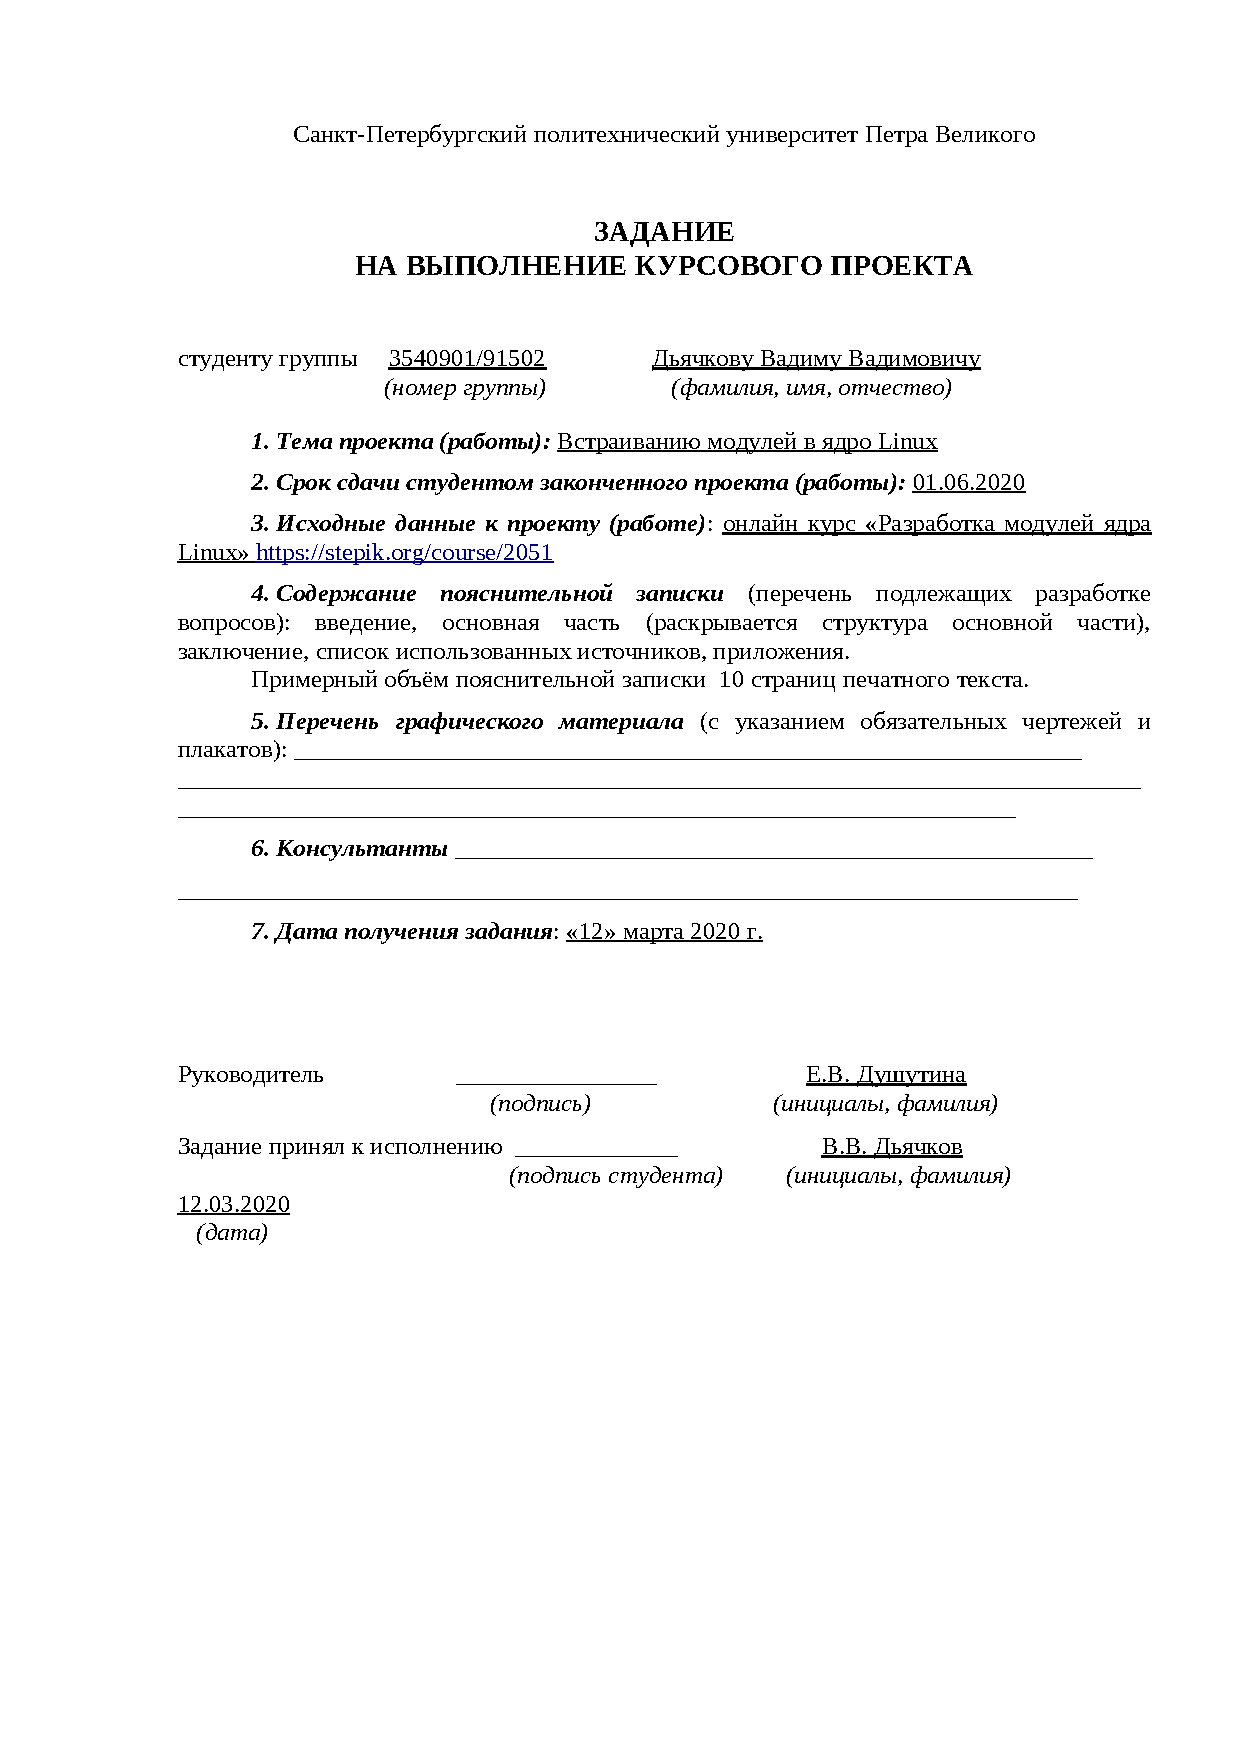
\includepdf[pages=-]{task.pdf}

%оформите отчет по встраиванию модулей в ядро на основе пройденногоon-line курса, приведите анализ результатов и ваше впечатление о раскрытии темы и соответствию совр. уровню. Приведите свой обзор литературы на эту тему

\section{Введение}

Несмотря на то, что ядро операционной системы Linux является монолитным, оно позволяет выполнять динамическую вставку и удаление кода ядра в процессе работы. Загружаемый объект ядра называется модулем. Модуль по своей сути примерно то же, что и обычная программа. Модуль так же имеет точку входа и выхода и находится в своем бинарном файле. Но модули имеют непосредственный доступ к структурам и функциям ядра. Для программ в пространстве пользователя этот доступ ограничен библиотечными интерфейсами компилятора [4].

Загружаемый модуль ядра (LKM -- Loadable Kernel Module) -- объектный файл, содержащий код, расширяющий возможности ядра операционной системы [11]. Модули используются, чтобы добавить поддержку нового оборудования или файловых систем или для добавления новых системных вызовов. Когда функциональность, предоставляемая модулем, больше не требуется, он может быть выгружен, чтобы освободить память и другие ресурсы.

\begin{figure}[H]
	\centering
	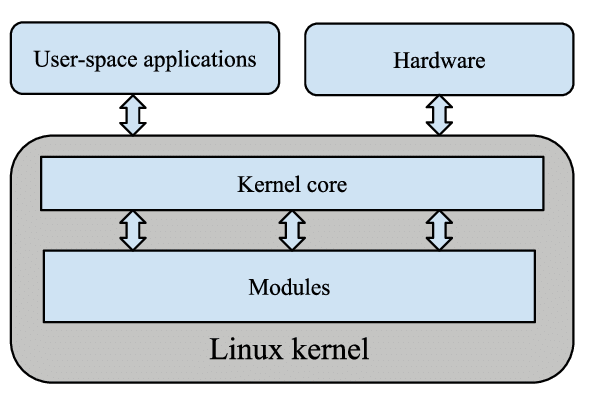
\includegraphics[width=0.6\linewidth]{module}
	\caption{Структура взаимодействия ядра с модулями}
\end{figure}

Без загружаемых модулей ядра операционные системы должны были бы иметь всю возможную функциональность в базовом ядре. Значительная часть кода не используется и лишь занимает память. Каждый раз, когда пользователю необходима новая функциональность, ещё не включенная в базовое ядро, требуется полная перекомпиляция базового ядра и перезагрузка. Использование подгружаемых модулей значительно упрощает изменение функциональности ядра и не требует ни полной перекомпиляции (модуль часто может быть собран отдельно от ядра или поставлен в предкомпилированном виде), ни перезагрузок [6].

\section{Онлайн-курс <<Разработка модулей ядра Linux>>}

Данный курс посвящен программированию в ядре Linux. В процессе курса освещается информация об архитектуре ядра, разработке драйверов простейших символьных устройств и принципах работы с внутренними структурами [3].

\subsection{<<Введение>>}

Теоретическая часть этого модуля знакомит слушателя с основными понятиями, связанными с разработкой ядра. Отдельными шагами выполняется скачивание исходных тестов ядра\footnote{\url{https://www.kernel.org/}}, конфигурирование при помощи команды \code{make menuconfig} и его сборка при помощи той же утилиты \code{make}.

Затем демонстрируется простейший модуль ядра, единственный задачей которого является логирование факта загрузки и выгрузки модуля. Это же задание для закрепления было в секции практических заданий:

\solutionlisting{1}{1}

Наиболее сложным заданием этого модуля оказалось создание модуля, который динамически выделяет необходимое количество памяти и освобождает ее при выгрузке. В данном случае демонстрируются особенности работы с памятью в ядре: вместо традиционных функций \code{malloc} и \code{free}, необходимо использовать \code{kmalloc} и \code{kfree}.

\solutionlisting{1}{4}

\subsection{<<Модули и файловые операции>>}

Данный модуль посвящен созданию драйвера символьного устройства. Для начала, описываются дополнительные сведения о модулях: возможность передачи параметров во встраиваемый модуль при помощи макросов, объявленных в \code{linux/moduleparam.h}. Данная функция позволяет параметризовать разработываемый модуль, например, путем до некоторого файла или устройства.

Затем лектор приводит базовую информацию о файловой системе \code{/dev}, которая используется в качестве точек входа для общения с устройствами из пространства пользователя: чтения и записи соответственно. Модуль создает в ядре специальную структуру \code{file_operations}, в которой регистрируются адреса функций, которые будут обрабатывать запросы на чтение и запись к соответствующей ноде в \code{/dev}. 

По итогам пройденного модуля был разработан модуля ядра, который реализует файловый интерфейс драйвера символьного устройства. Драйвер дополнительно ведет подсчет общего количества открытий символьного устройства и общего объема записанных в него данных. Эти данные также могут быть прочитаны с символьного устройства \code{/dev/solution_node}.

\solutionlisting{2}{2}

\subsection{<<Динамические ноды. Конфигурирование ядра>>}

Данный модуль посвящен созданию динамических нод в файловой системе \code{/dev}, а также доработке разработанного ранее драйвера символьного устройства для поддержки операций позиционирования и определения конца файла в хранящемся внутри модуля буфере.

Большое внимание также уделяется структура каталогов ядра в исходном коде. Выделим наиболее важные каталоги:
\begin{itemize}
	\item \code{/Documentation} -- объемная документация, описывающая все функции ядра;
	\item \code{/kernel} -- реализация базовых компонентов ядра (прерывания, планировщик, таймер и др.);
	\item \code{/fs} -- множество файловых систем, которые поддержаны в Linux;
	\item \code{/ipc} -- средства межпроцессного взаимодействия (очереди, разделяемая память и др.);
	\item \code{/include} -- заголовочные файлы, которые можно использовать при разработке модулей;
	\item \code{/drivers} -- исходный код различных драйверов устройств
\end{itemize}

По итогам изученного модуля, был доработан модуль ядра, который реализует файловый интерфейс драйвера символьного устройства. Драйвер выделяет отдельный участок памяти для каждого нового сеанса (для этого используется поле \code{private_data} структуры \code{file}) и поддерживает операции записи, чтения и изменение указателя текущей позиции \code{llseek} (при помощи высчитывания позиции внутри буфера). При этом разработанный драйвер обеспечивает корректную работу при параллельном выполнении этих операций за счет того, что для каждой сессии используется свой буфер данных.

\solutionlisting{3}{2}

\subsection{<<Списки. Прерывания. ioctl5>>}

Четвертый модуль посвящен трем основным темам -- структурам данных в ядре, прерываниям и таймерам.

В качестве базовой структуры данных в ядре часто используется двусвязный список, определенный в \code{linux/list.h}. Каждый элемент списка имеет указатель на следующий и предыдущий элемент, что позволяет удобно итерироваться между ними и производить вставку нового элемента в список.

Для закрепления навыков использования структур данных из ядра был разработан модуль, который выводит имена всех модулей в \code{kobject} с именем \code{/sys/kernel/my_kobject/my_sys}. Для этого используются используются функции \code{list_for_each} для итерации по массиву и \code{list_sort} для его сортировки. Стоит отметить, что данное API довольно удобно и легко использовать при разработке собственного модуля.

\solutionlisting{4}{1}

Прерывания являются асинхронными и связаны прежде всего с переферийными устройствами. Для обработки прерываний используется обработчик прерываний (ISR -- Interrupt Service Routine). Прерывания делятся на маскируемые и немаскируемые. Их отличие в том, что вторые нельзя отключить.

Другим важным заданием этого модуля было разработать модуль ядра, реализующий настройку и запуск нескольких таймеров по цепочке. Задержка запуска каждого таймера передается в модуль в виде параметра-массива в миллисекундах, а задержка для таймера номер N (начиная с нуля) в цепочке должна соответствовать N-ому значению в этом массиве. Для реализации используется несколько библиотечных функций: \code{ktime_set} для задания интервала времени, \code{hrtimer_start} для запуска таймера с установленной функцией обратного вызова (callback), которая будет вызвана по истечении времени таймера. Для сдвига таймера используется функция \code{hrtimer_forward_now}. При выгрузке модуля из ядра таймер выключается при помощи \code{hrtimer_cancel}.

\solutionlisting{4}{4}

\subsection{<<Дополнительные сведения>>}

Заключительный модуль начинается с информации о соглашениях, принятых при разработке ядра. К таким соглашениям относится стиль именования переменных, формат документирования своих функций, а также использование стандартных структур данных, рассмотренных в прошлом модуле.

Затем уделяется внимание примитивам синхронизации, которые используются для обеспечения корректности выполнения при параллельном выполнении запросов из различных модулей или пользователей. Выполняется обзор готовых атомарных операций, объявленных в \code{linux/atomic.h}. Эти операции могут быть использованы для построения более высокоуровневых примитивов синхронизации: спинлоки, мьютексы и семафоры.

\subsection{Впечатления от курса и обзор литературы}

В целом, после прохождения курса остались двоякие впечатления. С одной стороны, курс обладает массой достоинств. Во-первых, альтернативных онлайн-курсов, посвященных разработке модулей ядра Linux, в русскоязычном сегменте Интернета крайне мало. Во-вторых, курс тематически поделен на различные аспекты разработки модуля ядра, что позволяет в пройти путь от создания базового модуля <<hello world>> до модуля драйвера символьного устройства, который динамически создает ноды в \code{/dev} и поддерживает все базовые операции -- чтение, запись и позиционирование. В-третьих, платформа Stepik, на которой размещен курс, довольна удобна, позволяет обсудить лекции и задания в комментариях, а также задать вопрос лично команде курса.

Однако в курсе присутствуют и отрицательные моменты. Во-первых, часть теоретической информации не подкрепляется практическими заданиями (например, создание собственного прерывания и встраивание его в ядро). Во-вторых, часть информации, представленной в курсе, устарело в том или ином виде (например, в курсе рассказывает про Big Kernel Lock как один из подходов к синхронизации доступа в ядре, хотя этот механизм был удален еще в 2011 году [10]). Наконец, значительная часть информации является поверхностной и не создает полного впечатления о механизме работы модулей ядра Linux.

Отдельно стоит выделить литературу, связанную с тематикой курса. В первую очередь это книги Эндрю Таненбаума, посвященные фундаментальным основам разработки и проектирования операционных систем [2, 3]. В них читателя знакомят с базовыми принципами операционных систем. Также удачным изданием, с точки зрения практической части, кажется методическое пособие <<Системное программное обеспечение>> [1], содержащее как и теоретические основы ОС, так и практические упражнения. Что касается разработки модулей ядра, то эта тематика является довольно узкоспециализированной, тем не менее можно выделить несколько книг [5, 6, 7], посвященных исключительно разработке модулей ядра Liunx. В них гораздо более глубоко разбираются механизмы, которые используются внутри ядра и могут быть использованы при написании собственных модулей: таймеры, управление памятью, драйверы и др.

В сравнении с приведенной выше литературой, курс кажется довольно поверхностным и неглубоким, и носит скорее обзорный характер. Тем не менее, за счет практических заданий, у студента сохраняется возможность углубить свои знания в процессе их решения.

\newpage

\section{Заключение}

В рамках курсовой работы был рассмотрен механизм встраивания модулей в ядро Linux. Было представлено описание этого механизма, а также рассмотрены его основные применения.

На основе онлайн-курса <<Разработка модулей ядра Linux>> были продемонстрированы базовые функции модулей, а также реализовано несколько модулей ядра: драйвер символьного устройства, а также модули, использующие таймеры, списки и функции ввода-вывода. Несмотря на ряд минусов данного курса, отмеченных выше, благодаря курсу были как закреплены ранее изученные знания о модулях ядра, так и изучены новые функции и возможности, которые можно использовать в дальнейшем при разработке собственных компонентов операционной системы.

Исходный код модулей ядра, разработанных в процессе выполнения онлайн курса, доступен по ссылке в GitHub репозитории \footnote{\url{https://github.com/vaddya/operating-systems/tree/master/linux_kernel}}.

\newpage

\section*{Список использованных источников}

\begin{enumerate}
	\item Душутина Е.В. Системное программное обеспечение. Практические вопросы разработки системных приложений [Текст] -- 2016.
	\item Таненбаум Э. Современные операционные системы [Текст] -- 2015.
	\item Таненбаум, Э. Операционные системы. Разработка и реализация [Текст]. -- СПб.: Питер, 2006. -- 576 с.
	\item P. Raghavan et al. Emebedded Linux System Design and Development [Текст] -- 2006.
	\item B. Ward. How Linux Works, 2nd Edition: What Every Superuser Should Know [Текст] -- 2015.
	\item J. Corbet et al. Linux Device Drivers, 3rd Edition [Текст] -- 2005.
	\item Соловьев А. Разработка модулей ядра ОС Linux [Текст] -- 2015.
	\item Разработка модулей ядра Linux. Stepik [Электронный ресурс]. -- URL: \url{https://stepik.org/course/2051} (дата обращения: 25.04.2020)
	\item Загружаемый модуль ядра. Википедия [Электронный ресурс]. -- URL: \url{https://ru.wikipedia.org/wiki/%D0%97%D0%B0%D0%B3%D1%80%D1%83%D0%B6%D0%B0%D0%B5%D0%BC%D1%8B%D0%B9_%D0%BC%D0%BE%D0%B4%D1%83%D0%BB%D1%8C_%D1%8F%D0%B4%D1%80%D0%B0} (дата обращения: 31.05.2020)
	\item Giant lock. Wikipedia [Электронный ресурс]. -- URL: \url{https://en.wikipedia.org/wiki/Giant_lock} (дата обращения: 31.05.2020)
	\item Обзор архитектуры и возможностей системы Linux -- Интуит [Электронный ресурс]. -- URL: \url{https://www.intuit.ru/studies/courses/641/497/lecture/11314} (дата обращения: 31.05.2020)
\end{enumerate}

\end{document}
